% -*- mode: latex; -*- mustache tags:  
\documentclass[10pt,twoside,english]{_support/latex/sbabook/sbabook}
\let\wholebook=\relax

\usepackage{import}
\subimport{_support/latex/}{common.tex}

%=================================================================
% Debug packages for page layout and overfull lines
% Remove the showtrims document option before printing
\ifshowtrims
  \usepackage{showframe}
  \usepackage[color=magenta,width=5mm]{_support/latex/overcolored}
\fi


% =================================================================
\title{The Pillar Super Book Archetype Using Microdown}
\author{The Pillar team}
\series{Square Bracket tutorials}

\hypersetup{
  pdftitle = {The Pillar Super Book Archetype Using Microdown},
  pdfauthor = {The Pillar team},
  pdfkeywords = {project template, Pillar, Pharo, Smalltalk}
}


% =================================================================
\begin{document}

% Title page and colophon on verso
\maketitle
\pagestyle{titlingpage}
\thispagestyle{titlingpage} % \pagestyle does not work on the first one…

\cleartoverso
{\small

  Copyright 2017 by The Pillar team.

  The contents of this book are protected under the Creative Commons
  Attribution-ShareAlike 3.0 Unported license.

  You are \textbf{free}:
  \begin{itemize}
  \item to \textbf{Share}: to copy, distribute and transmit the work,
  \item to \textbf{Remix}: to adapt the work,
  \end{itemize}

  Under the following conditions:
  \begin{description}
  \item[Attribution.] You must attribute the work in the manner specified by the
    author or licensor (but not in any way that suggests that they endorse you
    or your use of the work).
  \item[Share Alike.] If you alter, transform, or build upon this work, you may
    distribute the resulting work only under the same, similar or a compatible
    license.
  \end{description}

  For any reuse or distribution, you must make clear to others the
  license terms of this work. The best way to do this is with a link to
  this web page: \\
  \url{http://creativecommons.org/licenses/by-sa/3.0/}

  Any of the above conditions can be waived if you get permission from
  the copyright holder. Nothing in this license impairs or restricts the
  author's moral rights.

  \begin{center}
    
\includegraphics[width=0.2\textwidth]{_support/latex/sbabook/CreativeCommons-BY-SA.pdf}
  \end{center}

  Your fair dealing and other rights are in no way affected by the
  above. This is a human-readable summary of the Legal Code (the full
  license): \\
  \url{http://creativecommons.org/licenses/by-sa/3.0/legalcode}

  \vfill

  % Publication info would go here (publisher, ISBN, cover design…)
  Layout and typography based on the \textcode{sbabook} \LaTeX{} class by Damien
  Pollet.
}


\frontmatter
\pagestyle{plain}

\tableofcontents*
\clearpage\listoffigures

\mainmatter


\part{My First book using Microdown}
\chapter{Compilation}
\begin{figure}[htpb]
\begin{center}

\includegraphics[width=0.3\textwidth]{/Users/ducasse/Workspace/FirstCircle/MyBooks/Bk-Writing/PharoBooks2/booklet-AdvancedMicroProjects/Chapters/Chapter1/figures/pillar.png}
\caption{Pillar logo}
\end{center}
\end{figure}


\section{Welcome to Pillar's little user-guide !!}
To write a book, you can create chapters and include them into \textcode{book.pillar}
or directly edit the file.
If you don't know ''Pillar'', check its documentation at \href{}{http://github.com/pillar-markup/pillar}\footnotesize{\url{}}

\chapter{Edition and Templates}
There is also a template system, you can find template in the folder \textcode{\_support/template}.
Some template are already written, but if you want to have your own, you had two solutions:

\begin{itemize}
    \item edit the existing template related to the format you want to change (recommanded)
    \item create your own template with its own name
\end{itemize}

You will found some template examples in \textcode{\_support/template} folder to see how it works.
The default template system is Mustache.

Output directory's default name is ''book-result'' but you can change it in the pillar.conf file by editing the\textcode{OUTPUTDIRECTORY} variable

\begin{figure}[htpb]
\begin{center}

\includegraphics[width=0.3\textwidth]{/Users/ducasse/Workspace/FirstCircle/MyBooks/Bk-Writing/PharoBooks2/booklet-AdvancedMicroProjects/Chapters/Chapter2/figures/pharo.png}
\caption{blue}
\end{center}
\end{figure}
\begin{figure}[htpb]
\begin{center}
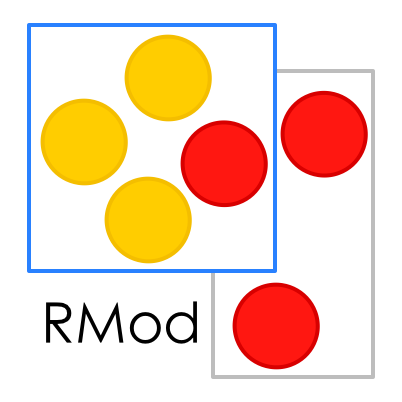
\includegraphics[width=0.3\textwidth]{/Users/ducasse/Workspace/FirstCircle/MyBooks/Bk-Writing/PharoBooks2/booklet-AdvancedMicroProjects/Chapters/Chapter2/figures/rmod.png}
\caption{jlklkjlk}
\end{center}
\end{figure}




\bibliographystyle{alpha}
\bibliography{book.bib}

% lulu requires an empty page at the end. That's why I'm using
% \backmatter here.
\backmatter

% Index would go here

\end{document}
